% Opcje klasy 'iithesis' opisane sa w komentarzach w pliku klasy. Za ich pomoca
% ustawia sie przede wszystkim jezyk oraz rodzaj (lic/inz/mgr) pracy.
\documentclass[shortabstract, english, inz]{iithesis}

\usepackage[utf8]{inputenc}

%%%%% DANE DO STRONY TYTUŁOWEJ
% Niezaleznie od jezyka pracy wybranego w opcjach klasy, tytul i streszczenie
% pracy nalezy podac zarowno w jezyku polskim, jak i angielskim.
% Pamietaj o madrym (zgodnym z logicznym rozbiorem zdania oraz estetyka) recznym
% zlamaniu wierszy w temacie pracy, zwlaszcza tego w jezyku pracy. Uzyj do tego
% polecenia \fmlinebreak.
\polishtitle    {Porównanie wydajności \fmlinebreak różnych implementacji algorytmu Wave Function Collapse}
\englishtitle   {Performance comparison of Wave Function Collapse Algorithm implementations}
\polishabstract {Algorytm Wave Function Collapse (WFC) autorstwa Maxim'a Gumin'a służy do proceduralnego tworzenia treści (ang. procedural content generation PCG) w oparciu o przykładowe obrazy i jest przykładem algorytmu probabilistycznego. Dla uzyskania podobieństwa pomiędzy danymi wejściowymi a wynikiem, algorytm składa obraz z fragmentów wejścia przestrzegając zasad sąsiedztwa z oryginalnego obrazu. Ten dokument opisuje zasady działania WFC, jego zastosowania i analizę wydajności różnych implementacji wariantu algorytmu służącego do tworzenia trójwymiarowego modelu w oparciu o zestaw klocków (ang. tileset) w tym moje autorskie pomysły na poprawę wydajności tego algorytmu.\fmlinebreak\url{https://github.com/KrzysiekSlawik/wfc}}
\englishabstract{Wave Function Collapse (WFC) algorithm by Maxim Gumin can be used for procedural content generation (PCG) and is an example of an probabilistic algorithm. It's input is example image and it's output is image following input style by using parts of example image and respecting neighbor relation between them. This paper aims at describing theory behind WFC, where it can be applied and performance comparison of implementations of WFC variant that serves as tilemap generator including my original ideas for performance improvement of the algorithm. \fmlinebreak\url{https://github.com/KrzysiekSlawik/wfc}}
% w pracach wielu autorow nazwiska mozna oddzielic poleceniem \and
\author         {Krzysztof Sławik}
% w przypadku kilku promotorow, lub koniecznosci podania ich afiliacji, linie
% w ponizszym poleceniu mozna zlamac poleceniem \fmlinebreak
\advisor        {dr Łukasz Piwowar}
\date          {03.02.2023}                     % Data zlozenia pracy
% Dane do oswiadczenia o autorskim wykonaniu
\transcriptnum {307020}                     % Numer indeksu
\advisorgen    {dr. Łukasza Piwowara} % Nazwisko promotora w dopelniaczu
%%%%%

%%%%% WLASNE DODATKOWE PAKIETY
%
%\usepackage{graphicx,listings,amsmath,amssymb,amsthm,amsfonts,tikz}
%
\usepackage{url}
\usepackage{graphicx}
\usepackage{float}
\usepackage{subcaption}
\usepackage[sorting=none]{biblatex}
\addbibresource{bibliography.bib}
%%%%% WŁASNE DEFINICJE I POLECENIA
%
%\theoremstyle{definition} \newtheorem{definition}{Definition}[chapter]
%\theoremstyle{remark} \newtheorem{remark}[definition]{Observation}
%\theoremstyle{plain} \newtheorem{theorem}[definition]{Theorem}
%\theoremstyle{plain} \newtheorem{lemma}[definition]{Lemma}
%\renewcommand \qedsymbol {\ensuremath{\square}}
% ...
%%%%%

\begin{document}

%%%%% POCZĄTEK ZASADNICZEGO TEKSTU PRACY

\chapter{Introduction}
This chapter briefly describes WFC, its background, roots, and use cases.
\section{Texture Synthesis}
\begin{figure}[H]
\centering
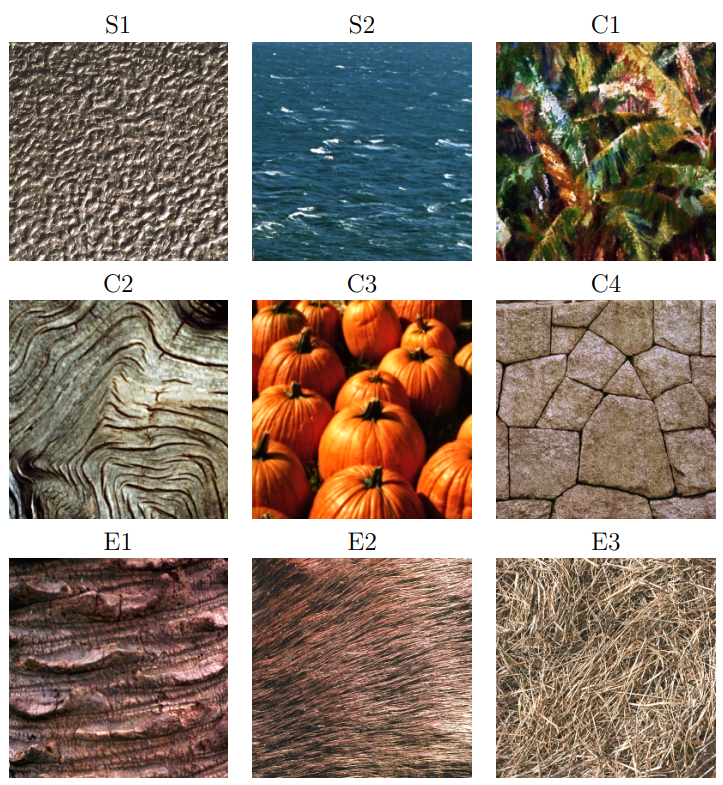
\includegraphics[width=0.75\textwidth, angle=0]{images/texsynth_input.png}
\caption{Input images for Patchwork texture synthesis (Source: \cite{harrison2002patchwork})}
\label{fig:texSynthIn}
\end{figure}
\begin{figure}[H]
\centering
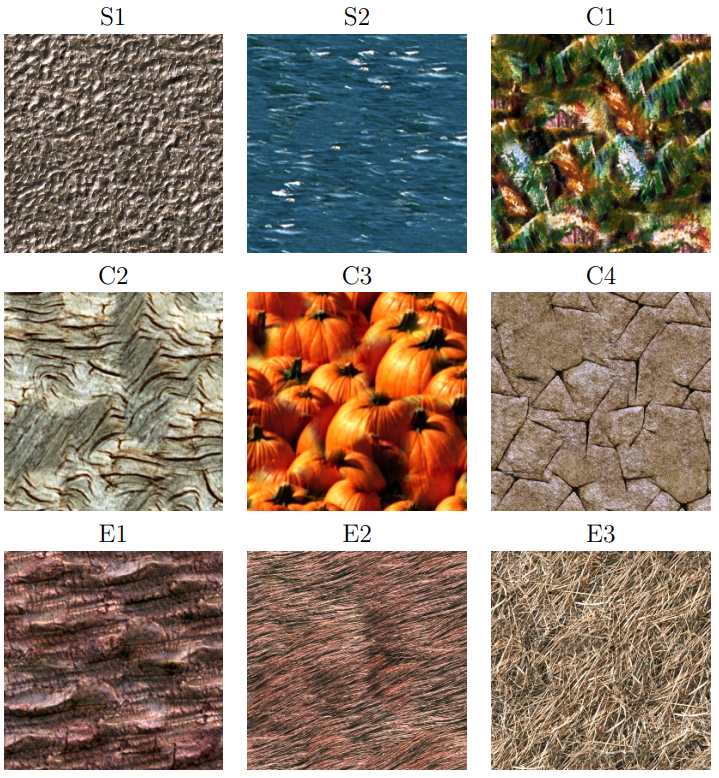
\includegraphics[width=0.75\textwidth, angle=0]{images/texsynth_output.png}
\caption{Output images for Patchwork texture synthesis (Source: \cite{harrison2002patchwork})}
\label{fig:texSynthOut}
\end{figure}
In computer graphics, texture synthesis is the problem of generating an output image that is bigger than the input image while resembling it. Most techniques solving this problem aim at having high similarity of patterns which are sub-images of small sizes (e.g. 5x5 pixels). It is worth mentioning that similarity, in most cases, is based on the Euclidean distance of pixel colors, whereas in the case of WFC, patterns have to be an exact match.\cite{Smith}
The requirement of exact match of patterns allows for much wider use of WFC than other typical texture synthesis tools as with little adjustments users can easily define key features of the output image. \cite{GraphBased}
\begin{figure}[H]
\centering
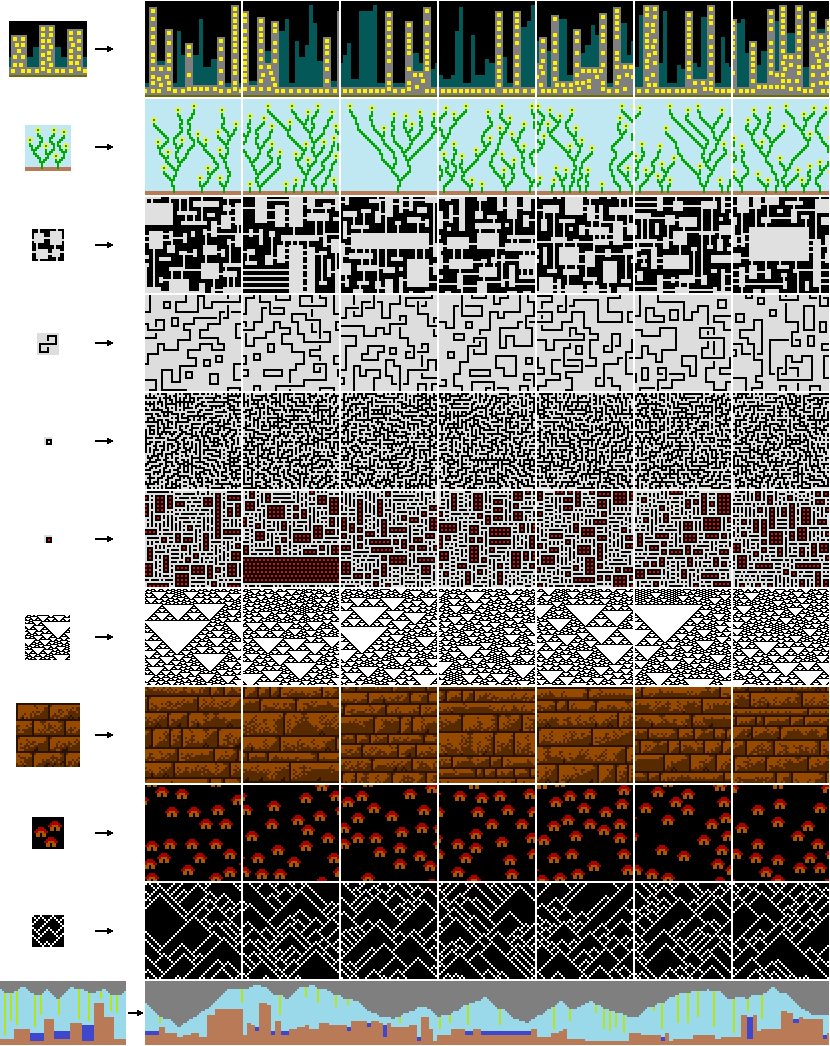
\includegraphics[width=0.75\textwidth, angle=0]{images/wfc.png}
\caption{Examples of inputs and outputs of the WFC algorithm (Source: \cite{MaximGumin})}
\label{fig:wfc}
\end{figure}
As stated by Maxim Gumin, WFC tends to be slower than P. F. Harrison's texture synthesis algorithm (examples see \ref{fig:texSynthIn} \ref{fig:texSynthOut}) but strict relation in which patterns have to be in images produced by WFC allows for capturing long correlations like a pattern of bricks, greenery or abstract shapes with a pixel perfect precision, which makes it the perfect candidate to use with pixel art and for level generation. See \ref{fig:wfc}.\cite{MaximGumin}


\section{Constraint Solving Algorithms}
\begin{figure}[H]
\centering
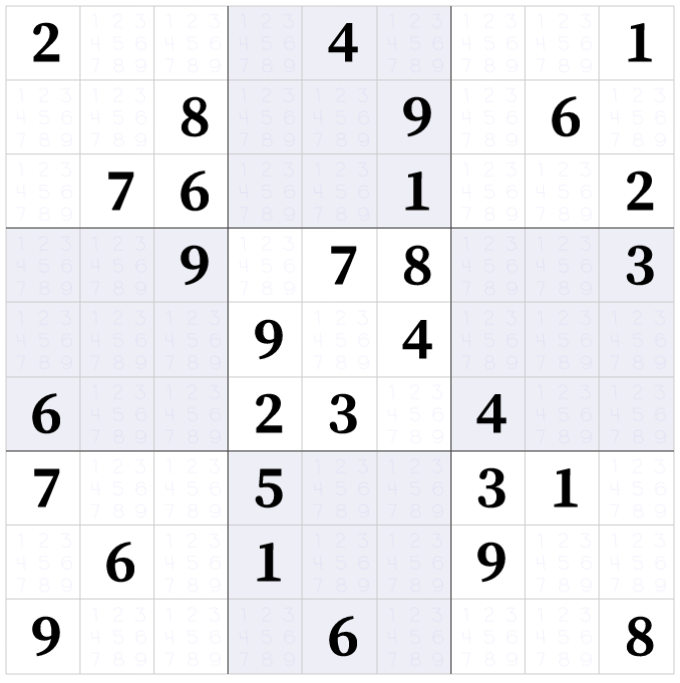
\includegraphics[width=0.75\textwidth, angle=0]{images/sudoku.png}
\caption{Example Sudoku problem (Source: \cite{sudoku})}
\label{fig:sudoku}
\end{figure}
Constraint satisfaction problems (CSPs) are typically defined in terms of decision variables and values. An example of CSP might be the Sudoku game (\ref{fig:sudoku}) in which each location on the grid is variable and values come from digits set. The goal of an algorithm solving CSPs is to find a total assignment (each variable has an assigned value) that does not violate any constraints. \fmlinebreak
WFC algorithm constructs the solution image by assigning values from a discrete set of unique local patterns from the input image. \cite{Smith} The key observation is that WFC being a CSP solver means that each iteration (every step of the algorithm that assigns to the variable) produces a new valid CSP. This can be used to guide WFC by assigning some variables by hand, as partially solved CSP is still proper input for any CSP solver. (as long as partial assignment does not violate constraints)
\section{Procedural Content Generation}
PCG is a powerful tool wherever a high or endless amount of content is required as PCG can reduce the resources spent on new assets by generating them based on those already manually created by artists or creating them entirely based on rules predefined in the algorithm. An important factor in deciding when to use PCG is the cost of the preparation algorithm compared with the cost of manually making all assets. In the case of products that require an endless amount of assets PCG is the only available option and it has to be a highly controlled process. The upfront cost of using PCG comes from choosing a well-fitted method, parameter tuning, deeply understanding the design, and knowing how to encode it.
From the game development point of view, two types of PCG can be distinguished. Offline PCG is used for creating assets during development, it doesn't have to produce output in real-time and its output can be checked by artists before being used in the final product. On the other hand, online PCG is used in the final application runtime. It has to work in real-time and produce its output in an acceptable loading screen time. Artists can't check algorithm outputs so it has to be highly controllable and fine-tuned during the development phase.\cite{DesignLevelConstraints}\break\break
WFC algorithm's main advantages in PCG are ease of use as basic results can be achieved by tuning input image only, high controllability as strict neighbor relations can guarantee the generation of playable content, easily extended by adding additional rules like density, total count, distance on top of neighbor relations. \cite{Smith, DesignLevelConstraints}

\section{Chapters Summary}
Summary of the following chapters:
\begin{itemize}
    \item \ref{chapter2}. WFC Applications - notable examples of how WFC might be used
    \item \ref{chapter3}. The WFC Algorithm - description and analysis of the original algorithm
    \item \ref{chapter4}. Performance Comparison - analysis of the performance of the WFC algorithm implemented by me, comparison of different used improvements
    \item \ref{chapter5}. Technical - how to install and test my code, technologies used
    \item \ref{chapter6}. Summary And Future Work - short description of obtained results and ideas for future development.
\end{itemize}



\chapter{WFC Applications}
\label{chapter2}
\section{level generation}
\begin{figure}[H]
\centering
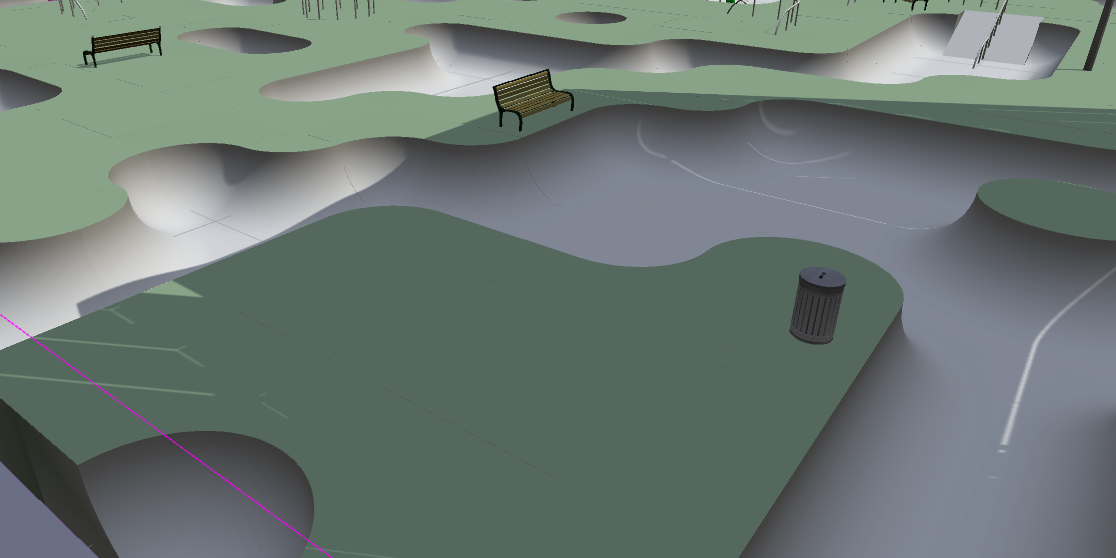
\includegraphics[width=0.75\textwidth, angle=0]{images/skater.png}
\caption{Proc Skater - the first game in which WFC was used for level generation (Source: \cite{skater})}
\label{fig:skater}
\end{figure}
WFC algorithm appeared in a game for the first time during the ProcJam event in form of a submission from Joseph Parker, Ryan Johns, and Oscar Morante - Proc Skater game \ref{fig:skater}. As stated by Joseph Parker, he has “never been this excited about an algorithm!”. In the case of their game use of WFC ensured smooth traversability of the level thanks to exact pattern matching used by the algorithm.\break
 Oskar Stålberg is another game developer that participated in the popularization of the WFC algorithm by creating a small demo web application\footnote{Demo of WFC by  Oskar Stålberg \url{http://oskarstalberg.com/game/wave/wave.html}}. He was one of the first to generalize WFC for other shapes and 3D meshes\footnote{WFC algorithm filling sphere surface with triangle shaped tiles by Oskar Stålberg \url{https://twitter.com/OskSta/status/784847588893814785}}. Oskar Stålberg also contributed by adding backtracking\ref{backtracking} and bitwise operations\ref{bitwise} as performance improvements.\cite{Smith}


\section{solving CSPs}
\begin{figure}[H]
\centering
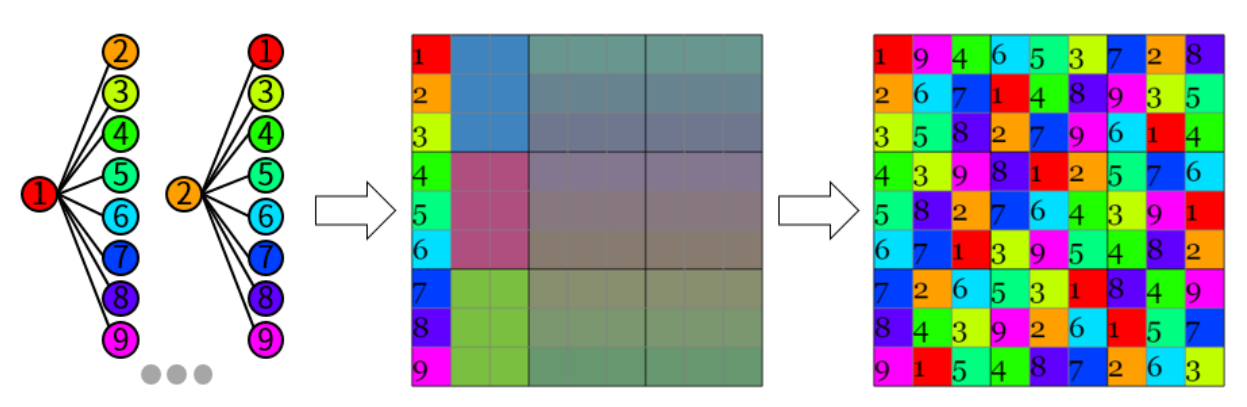
\includegraphics[width=1\textwidth, angle=0]{images/sudoku_solver.png}
\caption{Sudoku allowed neighbors, initial state, puzzle solved using graph-based WFC (Source: \cite{GraphBased})}
\label{fig:sudoku_solver}
\end{figure}
WFC algorithm can be used to solve CSPs if properly modified to fit the domain. An example would be solving the Sudoku game with WFC generalized for graphs which were done as a part of "Automatic Generation of Game Content using a Graph-based Wave Function Collapse Algorithm" \cite{GraphBased}. This paper focused on generalizing WFC by allowing each element to have a variable amount of neighbors but with the drawback of not distinguishing directions. \footnote{original WFC uses neighbor relations like "A is left neighbor of B" whereas, in case of the graph-based solution, we only know that "A is neighbor of B"} For solving the Sudoku game rules can be formulated in a way that fits this model - each variable has 20 neighbors.\ref{fig:sudoku_neighbors}.
\begin{figure}[H]
\centering
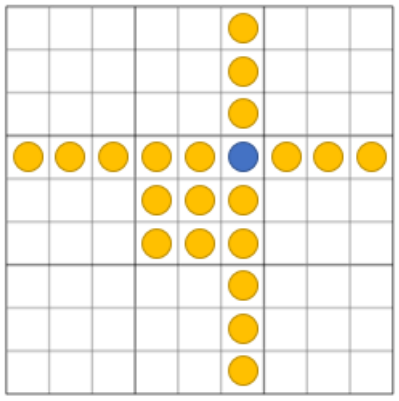
\includegraphics[width=0.50\textwidth, angle=0]{images/sudoku_neighbors.png}
\caption{blue represents selected Sudoku grid element, yellow represents its neighbors (Source: \cite{GraphBased})}
\label{fig:sudoku_neighbors}
\end{figure}
Backtracking \ref{backtracking}had to be added to WFC for it to be able to produce solutions for Sudoku puzzles as contradictions were common due to very strict rules. Even with backtracking WFC is not performing well as a CSP solver, but on the other hand, it can deduce the rules of the problem on its own.\cite{GraphBased}
\begin{figure}[H]
\centering
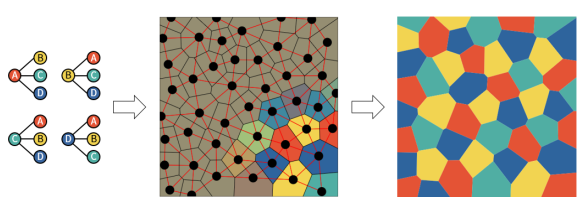
\includegraphics[width=1\textwidth, angle=0]{images/fourcolours.png}
\caption{Four Colours Problem being solved by WFC (Source: \cite{GraphBased})}
\label{fig:fourcolours}
\end{figure}
The same version of WFC was able to solve the four colors problem thanks to it being directly representable as a graph.\ref{fig:fourcolours} Algorithm was able to solve this CSP with basic rules of the four colors problem which it could deduce from the example solution, without any additional heuristics.\cite{GraphBased}


\section{writing poetry}
\begin{figure}[H]
\centering
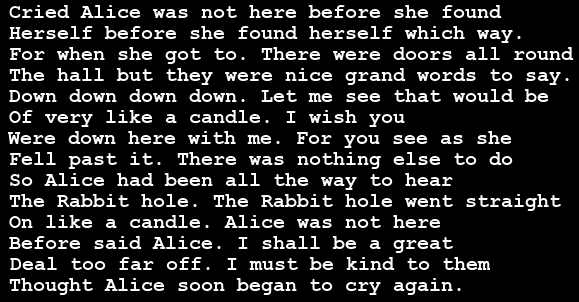
\includegraphics[width=1\textwidth, angle=0]{images/poem.png}
\caption{Poem written by Martin O’Leary WFC inspired algorithm (Source: \cite{wfcpoem})}
\label{fig:poem}
\end{figure}
One of the most unexpected contents generated with the WFC algorithm is poetry. Martin O’Leary inspired by Maxim Gumin's work decided to make WFC that enforced rhyme and meter constraints to generate poetry. Rhyme and meter constraints are long-distance constraints in opposition to the originally used neighbor constraints in the WFC algorithm. Tiles are created from syllables. Results can be seen in figure \ref{fig:poem}.\cite{Smith, wfcpoem}


\chapter{The WFC Algorithm}
\label{chapter3}
\section{pseudo code}
\begin{enumerate}
    \item Read the input bitmap and count NxN patterns.
    \item Create an array with the dimensions of the output (called "wave" in the source). Each element of this array represents a state of an NxN region in the output. A state of an NxN region is a superposition of NxN patterns of the input with Boolean coefficients (so a state of a pixel in the output is a superposition of input colors with real coefficients). A false coefficient means that the corresponding pattern is forbidden, true coefficient means that the corresponding pattern is not yet forbidden.
    \item Initialize the wave in the completely unobserved state, i.e. with all the boolean coefficients being true.
    \item \label{loop}Repeat the following steps:
    \begin{enumerate}
        \item Observation:
Find a wave element with minimal nonzero entropy. If there are no such elements (if all elements have zero or undefined entropy) then break the cycle (\ref{loop}) and go to step (\ref{final_step}).
Collapse this element into a definite state according to its coefficients and the distribution of NxN patterns in the input.
        \item Propagation: propagate information gained on the previous observation step.
    \end{enumerate}
    \item \label{final_step}By now all the wave elements are either in a completely observed state (all the coefficients except one being zero) or in a contradictory state (all the coefficients being zero). In the first case return the output. In the second case finish the work without returning anything.
\end{enumerate}
\cite{MaximGumin}

\section{deducing rules}
Patterns of size NxN are taken from the input image. Extra patterns can be generated from symmetries and rotations of original patterns. Every NxN part of the output image should belong to patterns deduced from the input image, thanks to this WFC can be used where pixel-perfect precision is required like a level generation or pixel arts.\cite{MaximGumin}
\section{observation}
The observation phase in the WFC algorithm handles two tasks - finds the lowest non-zero entropy\footnote{variable that can be assigned the least values but is not yet assigned} and collapses it \footnote{assigns value to the variable}.
Finding the lowest non-zero entropy in the original WFC implementation is done by simply searching through all variables looking for this with the least possible assignments. \cite{MaximGumin} This is good enough for small bitmaps but can be improved by introducing some kind of priority queue supporting the decrease key operation. More about this improvement can be read here \ref{fibheap} and here \ref{prioritybuckets}.
\section{propagation}
The propagation phase in the WFC algorithm handles updating possible assignments for each variable. Possible assignments have to be based on constraints given by possible values of neighbors. Possible values set is an intersection of allowed values from each neighbor and allowed values from every neighbor is the union of possible values for each legal assignment. It is quite intuitive to implement possible values as some kind of set, but it's important to notice that we need to make a lot of union and intersection operations.\break
The original implementation uses Boolean vectors of domain length, where each value represents if the value is legal. Maxim Gumin wrote his algorithm in C\# which Boolean vectors are specialized to store Boolean value in a single bit, but it is not specified by language if there are any optimizations for a series of logic operations, more over many programming languages do not have specialized Boolean vectors. More about data structure for storing variable possible assignments can be found here \ref{bitwise}.\break
The simplest solution would update all possible variable assignments as long as the system is not stable, however, it is important to note that updating the variable might require an update of each of its neighbors. (updates of variables happen both due to observation and propagation) This makes the propagation phase quite expensive and an obvious candidate for optimizations. The stack can be used to maintain elements that require updating. (as WFC author did in his implementation\ref{stack}) Similarly, the queue can be used\ref{queue}. A comparison of both solutions can be found here \ref{stack_vs_queue}.
\section{backtracking}
\label{backtracking}
In the original WFC implementation, there is no backtracking, if a contradiction is detected, the algorithm will just retry the whole generation process. Isaac Karth and Adam M. Smith showed in their work that the contradiction rate is dependent on how strict are the rules for assignments. In simple examples shown by Maxim Gumin, the contradiction rate is low enough not to use backtracking but for larger scale problems with more heuristics, the backtracking becomes crucial for the WFC to work correctly.
\cite{Smith}



\chapter{Performance Comparison}
\label{chapter4}
For performance comparison purposes I've created x versions of WFC in the rust programming language. From the performance point of view the deducing rules phase is not interesting and as a result, is skipped. Instead, input to the algorithm is a tile set with constraints and a tilemap to fill. (it can be partially assigned) I've been running benchmarks on tile set with relaxed restrictions\footnote{each tile has a high number of allowed neighbors}. To eliminate contradictions, the tile set contains tile that can be the neighbor of any other tile. I've added that special tile to make benchmarks more stable.\break
To ensure the correctness of all solutions, I've created tests that checked if the output followed the given rules. It's important to note that in the case of probabilistic algorithms, these kinds of tests have to be run multiple times to ensure correctness.\break
I've used the Criterion\footnote{A statistics-driven micro-benchmarking library written in Rust \url{https://docs.rs/criterion/latest/criterion/}} library for benchmarking all implementations.
For profiling I've used perf\footnote{about perf \url{https://perf.wiki.kernel.org/index.php/Main_Page}} with flamegraph\footnote{cargo flamegraph - the flamegraph generator written in rust \url{https://github.com/flamegraph-rs/flamegraph}}
    \section{baseline}
        \subsection{code analysis}
        \subsection{performance}
        \subsection{potential improvements}
    \section{Boolean vectors as representation of states \fmlinebreak similar to Maxim Gumin implementation from 2016}
        \subsection{code analysis}
        \subsection{performance}
        \subsection{applied improvements}
    \section{Stack maintaining elements that should be propagated next \fmlinebreak similar to Maxim Gumin current implementation}
    \label{stack}
        \subsection{pseudo code}
        \subsection{performance}
        \subsection{applied improvements}
    \section{Queue maintaining elements that should be propagated next}
    \label{queue}
        \subsection{pseudo code}
        \subsection{performance}
        \subsection{comparison with WFC version using stack}
        \label{stack_vs_queue}
    \section{bit vector as representation for states}
        \label{bitwise}
        \subsection{code analysis}
        \subsection{performance}
        \subsection{potential improvements}
    \section{Fibonacci Heap for faster finding of lowest non-zero entropy}
    \label{fibheap}
    This kind of improvement can reduce time complexity from linear to amortized logarithmic for removing minimum and constant for the decrease key operation.
        \subsection{code analysis}
        \subsection{performance}
        \subsection{potential improvements}
    \section{custom structure for faster finding of lowest non-zero entropy implementing decrease key operation}
    \label{prioritybuckets}
        \subsection{comparison with Fibonacci heap}
    \section{summary}
\chapter{Technical}
\label{chapter5}
    \section{installation instruction}
    \section{technologies used}
\chapter{Summary and Future Work}
\label{chapter6}

%%%%% BIBLIOGRAFIA

%%%%% BIBLIOGRAFIA
\printbibliography[sorting=none]

\end{document}
